\documentclass[10pt]{report} 
\usepackage{blindtext} 
\usepackage{times} 
\usepackage{graphicx} 
\usepackage[headheight=0pt,headsep=0pt]{geometry}
\usepackage{sectsty} 
\usepackage{float} 
\usepackage{array} 
\usepackage[backend=biber,bibencoding=latin1]{biblatex} 
\chapterfont{\centering} 
\usepackage{enumitem} 
\usepackage{enumerate} 
\usepackage{listings} 
\usepackage{color} 
\usepackage{ragged2e}
\usepackage{pdfpages}
\usepackage{titlesec}
\titlespacing*{\chapter}{-10pt}{-60pt}{-20pt}
\usepackage[headheight=0pt,headsep=0pt]{geometry} 
\definecolor{dkgreen}{rgb}{0,0.6,0} 
\definecolor{gray}{rgb}{0.5,0.5,0.5} 
\definecolor{mauve}{rgb}{0.58,0,0.82} 
\usepackage[table]{xcolor}
\definecolor{lightblue}{HTML}{ADD8E6}

\makeatletter
\def\@makechapterhead#1{%
  {\parindent \z@ \centering\normalfont
    \ifnum \c@secnumdepth >\m@ne
        \huge\bfseries \@chapapp\space \thechapter
        \par\nobreak
        \vskip 20\p@
    \fi
    \interlinepenalty\@M
    \Huge \bfseries #1\par\nobreak
    \vskip 40\p@
  }}
\def\@makeschapterhead#1{%
  {\parindent \z@ \centering
    \normalfont
    \interlinepenalty\@M
    \Huge \bfseries  #1\par\nobreak
    \vskip 40\p@
  }}
\makeatother
 
\lstset{ %   
language=Java,                % the language of the code  
 basicstyle=\footnotesize,           % the size of the fonts that are used for the code   numbers=left,                   % where to put the line-numbers   numberstyle=\tiny\color{gray},  % the style that is used for the line-numbers   stepnumber=1,                   % each line is numbered 
  numbersep=5pt,                  % how far the line-numbers are from the code 
  backgroundcolor=\color{white},      % choose the background color. You must add \usepackage{color}   
showspaces=false,               % show spaces adding particular underscores   showstringspaces=false,         % underline spaces within strings   
showtabs=false,                 % show tabs within strings adding particular underscores   frame=single,                   % adds a frame around the code 
  rulecolor=\color{black},        % if not set, the frame-color may be changed on line-breaks within notblack text (e.g. commens (green here)) 
  tabsize=2,                      % sets default tabsize to 2 spaces   captionpos=b,                   % sets the caption-position to bottom   breaklines=true,                % sets automatic line breaking   breakatwhitespace=false,        % sets if automatic breaks should only happen at whitespace   title=\lstname,                   % show the filename of files included with \lstinputlisting; 
                                  % also try caption instead of title   
keywordstyle=\color{blue},          % keyword style   commentstyle=\color{dkgreen},       % comment style  
 stringstyle=\color{mauve},         % string literal style  
 escapeinside={\%*}{*)},            % if you want to add a comment within your code   morekeywords={*,...}               % if you want to add more keywords to the set 
} 
\geometry{a4paper,total={180mm,250mm},left=20mm,top=20mm, right=20mm} 
\usepackage{indentfirst} 
\thispagestyle{empty} 
\begin{document} 
\newpage
\begingroup
\pagecolor{lightblue} % Set background to black
\color{black}     % Set all text to white
\thispagestyle{empty}

\begin{center}
    \LARGE{\textsc {\textbf{Smart Campus Event Management System}}}\\[0.2cm]
    \vspace{.5cm}
    \Large{\textit{\\School of Computing}}\\[0.3cm]
    
    \Large{\textbf{\\Bachelor of Technology\\in \\Computer Science \& Engineering}}
    \vspace{.5cm}
    \Large{\textbf{\\By}}\\[0.5cm]
    
    \begin{table}[h] 
    \centering 
    \Large{\color{red} % Ensure table text is white
    \begin{tabular}{>{\bfseries} lc>{\bfseries}r} J.Umesh (VTU25839)\\ 
    \end{tabular}} 
    \end{table} 

    \vspace{.5cm}
    \large{\textit{10211CS224}}\\ 
    \large{\textit{Full Stack Application Development\\ Slot : E2-B1}}\\ 
    \vspace{1cm} 

    
    % Logo with white stroke/border
    \fboxsep=5pt % Adjust border padding
   {\includegraphics[scale=0.5]{Logo.png}}\\ 
    
    \vspace{1.5cm}
    \large{\textbf{DEPARTMENT OF COMPUTER SCIENCE AND ENGINEERING}}\\ 
    \large{\textbf{SCHOOL OF COMPUTING}}\\ 
    \vspace{1cm}
    \Large{\textbf{VEL TECH RANGARAJAN Dr.SAGUNTHALA R\&D INSTITUTE OF SCIENCE AND TECHNOLOGY\\ (Deemed to be University Estd u/s 3 of UGC Act, 1956)}}\\ 
    \large{\textbf{CHENNAI 600 062, TAMILNADU, INDIA}} 
    \vspace{1cm}
    \large{\textbf{\\April, 2026}}\\ 
\end{center} 
\clearpage
\nopagecolor % Revert background to white for the rest of the document
\color{black} % Revert text to black for the rest of the document
\endgroup
 
%CERTIFICATE 
\newpage 
\pagenumbering{roman} 
\begin{center} 
{\Huge \textbf{ BONAFIDE CERTIFICATE}}\\[0.5cm] 
\end{center} 
\linespread{1.5} 
\large{It is certified that the work contained in the Full Stack Application Development report titled "Smart Campus Event Management System" by J.Umesh (VTU25839) has been carried out in Winter semester of Academic year 2025-2026(WS2526).} 
\vspace{1.5cm} 
\begin{flushright} 
\textbf{Signature of Faculty\\Dr. Chidambaranathan C M.
\\Associate Professor\\Computer Science \& 
Engineering\\School of Computing\\Vel Tech Rangarajan Dr.Sagunthala R\&D\\Institute of Science and Technology\\April, 2026}\\[2.0cm] 
\textbf{Signature of Course Coordinator\\Dr. Sumithra. M\\ Assistant Professor(Senior Grade) \\Computer Science \& Engineering\\School of Computing\\Vel Tech Rangarajan Dr.Sagunthala R\&D\\Institute of Science and Technology\\April, 2026}\\  
\end{flushright} 
 
%declaration 
\newpage 
\begin{center} 
\Huge \textbf{DECLARATION} 
\end{center} 
\linespread{1.5} 
\large{ 
 I declare that this written submission represents my ideas in my own words and where others' ideas or words have been included, we have adequately cited and referenced the original sources. I also declare that i have adhered to all principles of academic honesty and integrity and have not misrepresented or fabricated or falsified any idea/data/fact/source in our submission. I understand that any violation of the above will be cause for disciplinary action by the Institute and can also evoke penal action from the sources which have thus not been properly cited or from whom proper permission has not been taken when needed.} 
\vspace{2.0cm} 
\begin{flushright} 
\\ 
\large{J.Umesh}\\ 
\large{Date:\hspace*{1.0cm}/\hspace*{1.0cm}/}\\[2.0cm]
\\ 
\large{}\\ 
\large{}\\[2.0cm] 
\\ 
\large{}\\ 
\large{}\\[2.0cm] 
\end{flushright} 

 

%ABSTRACT 
\newpage 
\begin{center} 
\vspace{2cm} 
\Huge{\textbf{ABSTRACT}}\\[0.5cm] 

\end{center} 
\begin{center} 

\addtocontents{toc}{~\hfill\textbf{Page.No}\par} 

\addcontentsline{toc}{chapter}{ABSTRACT} 
\addtocontents{toc}{\protect\thispagestyle{empty}} 
\end{center} 
\Large{\paragraph  \\ }
 The Smart Campus Event Management System is an advanced digital solution designed to automate and enhance the process of organizing and managing events within an academic campus. Built using a robust technology stack including Java Spring Boot, Spring Data JPA, Thymeleaf, and MySQL, this platform offers a seamless and responsive experience for both event administrators and students.

A key innovation in this system is the integration of an interactive campus mapping feature powered by Leaflet.js. This allows students to visualize event locations geographically on the campus, providing an engaging and highly intuitive way to discover upcoming events. The system offers an interface for event creation, registration, and capacity management, enabling organizers to publish event details, set participant limits, and pinpoint geographic locations efficiently.

By providing real-time data handling and interactive components, the platform reduces manual workload, prevents scheduling conflicts, and streamlines student engagement across the campus.

\noindent \textbf{Keywords:} \textit{Smart Campus, Spring Boot, Event Management System, Campus Automation, Leaflet.js, Geographic Mapping, Online Registration, Thymeleaf, MySQL, Web-Based Application}
  
\textbf{} 
%list of figure 
\renewcommand*\listfigurename{LIST OF FIGURES} 

\addcontentsline{toc}{chapter}{LIST OF FIGURES} 
\listoffigures 
\renewcommand{\listtablename}{LIST OF TABLES}
\addcontentsline{toc}{chapter}{LIST OF TABLES}

\listoftables
 
%list of abbreviation 
\clearpage   % better than \newpage

\chapter*{\centering LIST OF ACRONYMS AND ABBREVIATIONS}
\addcontentsline{toc}{chapter}{LIST OF ACRONYMS AND ABBREVIATIONS}

\vspace{-1cm}   % remove extra gap

\begin{flushleft}

\textbf{API} \hspace{1.8cm} Application Programming Interface \\[0.3cm]
\textbf{CSS} \hspace{1.8cm} Cascading Style Sheets \\[0.3cm]
\textbf{DBMS} \hspace{1.4cm} Database Management System \\[0.3cm]
\textbf{HTML} \hspace{1.5cm} HyperText Markup Language \\[0.3cm]
\textbf{HTTP} \hspace{1.5cm} HyperText Transfer Protocol \\[0.3cm]
\textbf{JPA} \hspace{1.8cm} Java Persistence API \\[0.3cm]
\textbf{MVC} \hspace{1.8cm} Model-View-Controller \\[0.3cm]
\textbf{REST} \hspace{1.5cm} Representational State Transfer \\[0.3cm]
\textbf{SCEMS} \hspace{1cm} Smart Campus Event Management System \\[0.3cm]
\textbf{SQL} \hspace{1.8cm} Structured Query Language \\[0.3cm]
\textbf{UI/UX} \hspace{1.3cm} User Interface / User Experience \\

\end{flushleft}
\renewcommand*\contentsname{TABLE OF CONTENTS} 
%\addtocontents{toc}{\textbf{CONTENT} \hfill \textbf{PAGE NO.}} 
   
\tableofcontents 

\addtocontents{toc}{\protect\pagestyle{empty}} 
\thispagestyle{empty} 
 
%introduction 
\chapter{INTRODUCTION} 
\pagenumbering{arabic} 
\section{Introduction}
	The Smart Campus Event Management System is a modern web-based application built to streamline and automate the management of events within an educational institution. In traditional campus environments, event organization is often carried out manually using paper-based methods, emails, and informal communication channels. These approaches are time-consuming, prone to errors, and lack proper coordination, which can lead to scheduling conflicts, miscommunication, and inefficient resource utilization. 

Leveraging modern full-stack technologies like Java Spring Boot for robust backend logic and Thymeleaf for dynamic frontend rendering, this system provides an integrated platform where students, faculty, and administrators can collaborate effectively. It allows event organizers to create, update, and manage event details such as date, time, capacity limits, and venue locations.

A major feature of this system is the integration of an interactive geographical mapping component. Using Leaflet.js, upcoming events are pinned directly onto a digital campus map, allowing students to visually explore what is happening across the campus. In addition to simplifying event coordination, the system enhances the user experience by offering features such as automated capacity enforcement and secure data processing, ensuring transparent and accessible event management.
\linespread{1.5} 
\section{Aim of the Project} 
The main aim of the Smart Campus Event Management System is to develop an efficient, reliable, and user-friendly web application that automates the entire process of managing events within a campus. The project seeks to eliminate the limitations of traditional manual systems and replace them with a responsive digital solution that enhances productivity and coordination.

A key objective is to provide an immersive discovery experience. By integrating geographic mapping technologies (Leaflet.js), the system aims to present events visually, making it easier for students to find events based on campus locations. 

Another important aim is to enforce strong backend business rules to manage event capacities seamlessly. The platform ensures data consistency and prevents over-registration by verifying available slots in real-time. The system also focuses on offering a scalable backend architecture powered by Spring Boot and a structured MySQL database capable of handling growing volumes of data and concurrent user requests.

\section{Scope of the Project} 
The scope of the Smart Campus Event Management System encompasses the design, development, and implementation of a full-stack web application tailored for managing academic and cultural events on campus. It is designed to serve administrators, event organizers, and student participants.

Within its scope, the system provides functionalities such as event creation, editing, and geographical plotting. Organizers can define event details, establish geographical coordinates (latitude and longitude), set registration capacities, and monitor student enrollment. Participants can browse the interactive map or a detailed event list, register for events seamlessly, and view their registration status.

The system relies on a secure relational database schema for maintaining normalized data records of all events and registrations. While the platform focuses intensely on providing robust internal management and geographical discovery within the campus network, it does not currently encompass external payment gateways or large-scale public ticketing features.

\section{Framework} 
The Smart Campus Event Management System is built using a structured Model-View-Controller (MVC) framework that ensures efficient development, scalability, and maintainability. This multi-tier architecture separates the application into distinct layers, improving system organization and performance.

The presentation layer is developed using HTML, CSS, JavaScript, and Thymeleaf. Thymeleaf is used for server-side template rendering, tightly coupling the view layer with the Spring backend. The Leaflet.js library is employed on the client side to render the interactive geographic map and plot event markers dynamically based on data fetched from RESTful APIs.

The application logic layer handles the core functionalities, including event management, validation, and registration processing. This layer is implemented using Java and the Spring Boot framework. It processes user requests, executes business rules, and communicates seamlessly with the database using Spring Data JPA.
\begin{figure}[H]
\centering
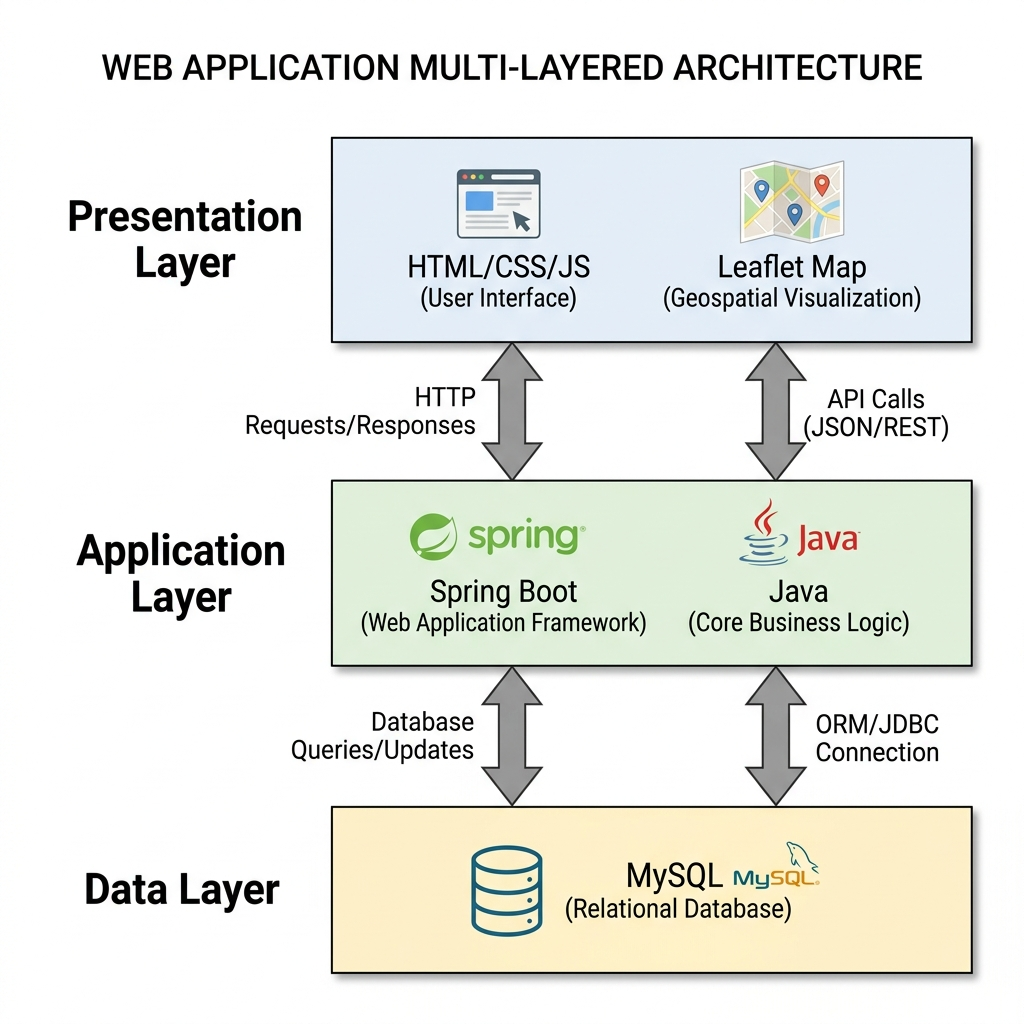
\includegraphics[scale=0.3]{Framework_Diagram.png}
\caption{Framework Diagram}
\label{fig:LIFI}
\end{figure}

Fig 1.1 illustrates the framework of the Smart Campus Event Management System, showcasing the structured multi-layered architecture. At the top level, users interact with the frontend views (Thymeleaf and Leaflet map). These interactions trigger HTTP requests to the Spring Boot controllers, which interact with the service layer to process logic, eventually interacting with the MySQL database through Spring Data JPA repositories.


\chapter{SURVEY OF SIMILAR APPLICATION IN MARKET} 

This section presents an overview of existing event management applications available in the market. These applications provide various features for organizing, managing, and analyzing events. However, most of them are designed for large-scale or commercial use and may not fully meet the specific interactive geographical requirements of a campus environment.

\subsection*{1. Whova}
Whova is an all-in-one event management platform widely used for conferences and professional events. It provides features such as event registration, attendee networking, live polling, and analytics. Although it offers advanced functionalities, it is often complex and may not be suitable for small-scale campus events.

\subsection*{2. Eventbrite}
Eventbrite is a popular global platform that allows users to create, promote, and manage events. It supports ticket booking and payment integration, making it easy to handle large audiences. However, it is primarily designed for public events and lacks customized interactive campus mapping for internal campus use.

\subsection*{3. Eventify}
Eventify is an end-to-end event management solution that includes features like registration, live Q\&A sessions, and analytics dashboards. It enhances attendee engagement but may not provide sufficient customization for educational institutions.

\subsection*{4. Eventzilla}
Eventzilla focuses on event registration and ticketing services. It allows organizers to create custom event pages and manage payments efficiently. However, it mainly concentrates on ticketing and does not provide comprehensive campus event management features.

\subsection*{5. Cvent}
Cvent is an enterprise-level event management system that supports venue management, budgeting, and marketing tools. It is highly suitable for large organizations but is expensive and complex for campus-level applications.

\subsection*{6. LineUpr}
LineUpr is an event engagement application that provides real-time notifications, schedules, and networking features. While it improves participant interaction, it lacks full-scale event management capabilities.

\subsection*{7. Blackthorn}
Blackthorn is a university-focused event management system built on the Salesforce platform. It offers features like registration, QR-based check-in, and analytics. Although it is tailored for educational institutions, it requires integration with Salesforce, which can be costly and complex.

\subsection*{Conclusion}
From the above survey, it is evident that most existing applications focus on large-scale or commercial event management. They often lack the specific feature of an interactive, geographical campus-based visual map for event discovery. Therefore, there is a need for a dedicated Smart Campus Event Management System that incorporates modern web technologies, spatial visualization (Leaflet.js), and robust backend processing (Spring Boot) specifically tailored for a university setting.

\linespread{1.5} 
 \begin{table}[h]
\centering
\caption{Comparison of Existing Event Management Applications}

\resizebox{\textwidth}{!}{
\begin{tabular}{|l|l|l|l|l|}
\hline
\textbf{Application} & \textbf{Type} & \textbf{Key Features} & \textbf{Advantages} & \textbf{Limitations} \\ \hline

Whova & Conference App & Registration, Networking, Analytics & Interactive, Feature-rich & Complex for small use \\ \hline

Eventbrite & Ticketing Platform & Event creation, Ticket booking, Payments & Easy to use & Not campus-specific, no map \\ \hline

Cvent & Enterprise System & Venue mgmt, Marketing, Analytics & Scalable, powerful & Expensive \\ \hline

Eventify & Event Platform & Q\&A, Registration, Dashboard & Real-time engagement & Limited customization \\ \hline

Eventzilla & Registration Tool & Ticketing, Custom pages & Flexible pricing & Focus on ticketing only \\ \hline

LineUpr & Engagement App & Notifications, Schedules & Good user interaction & Limited management features \\ \hline

Blackthorn & University System & QR check-in, Analytics & Campus-focused & Requires Salesforce \\ \hline

\textbf{SCEMS (Ours)} & \textbf{Campus System} & \textbf{Leaflet Map, Event Registration} & \textbf{Intuitive visual discovery} & \textbf{Restricted to Campus scope} \\ \hline

\end{tabular}
}

\end{table}

\chapter{FRAMEWORK DESCRIPTION} 

\section{Frontend Implementation}

\subsection{Environment Setup}
The frontend of the Smart Campus Event Management System is developed using modern web technologies alongside server-side rendering to provide an interactive interface. The core technologies include HTML, CSS, JavaScript, and Thymeleaf for template processing. A significant addition is the Leaflet.js library, which powers the interactive campus map.

Dependencies such as Bootstrap for responsive styling and Leaflet.js for mapping are included via Content Delivery Networks (CDNs). The frontend is tightly integrated with the Spring Boot application, processing dynamic model data passed from the backend controllers directly into the HTML views.

\subsection{Structure of the Project}
The frontend files reside within the \texttt{src/main/resources/} directory of the Spring Boot project. The \texttt{templates/} folder holds the Thymeleaf HTML files (e.g., \texttt{events.html}, \texttt{register.html}, \texttt{dashboard.html}). The \texttt{static/} folder stores the CSS stylesheets, JavaScript files, and images. 

JavaScript is utilized specifically to initialize the Leaflet map on the events page, fetching spatial data (latitude and longitude) to dynamically place markers that represent upcoming events.

\subsection{Execution Procedure}
When the Spring Boot application is executed, the embedded Tomcat server starts up. Users access the application via a web browser by navigating to the designated localhost port (e.g., \texttt{localhost:8080}). The server processes the request, populates the Thymeleaf templates with data from the database, and serves the fully rendered HTML to the client browser. 

% -----------------------------------------------------

\section{Backend Implementation}

\subsection{Environment Setup}
The backend is developed using Java and the Spring Boot framework to handle business logic, data validation, and communication with the database. The environment setup includes configuring the Java Development Kit (JDK) and using Maven as the build automation tool. 

The \texttt{pom.xml} file is configured with necessary dependencies including Spring Web, Spring Data JPA, MySQL Connector, and validation libraries. The \texttt{application.properties} file is used to define database connection strings and server port configurations.

\subsection{Structure of the Project}
The backend project adheres to the Model-View-Controller (MVC) architectural pattern. It is structured into distinct packages:
\begin{itemize}
    \item \textbf{Models:} Contains JPA entity classes (\texttt{Event}, \texttt{Registration}) mapped directly to the database tables.
    \item \textbf{Repositories:} Contains interfaces extending \texttt{JpaRepository} for abstracted CRUD operations.
    \item \textbf{Services:} Implements core business logic, such as checking event capacity limits before confirming a registration.
    \item \textbf{Controllers:} Manages HTTP requests and routes them to the appropriate services, returning populated Thymeleaf views or REST JSON responses.
\end{itemize}

\subsection{Execution Procedure}
To execute the backend, the main \texttt{EventManagementApplication} class is run as a Spring Boot App. The application automatically configures the database connection based on the properties file, executes any schema updates through Hibernate, and begins listening for incoming HTTP requests on the embedded server.

% -----------------------------------------------------

\section{Database Implementation}

\subsection{Database Configuration}
The database is configured to store and manage all core system data, primarily focusing on events and registrations. MySQL is utilized as the relational database management system. Connection details, including the JDBC URL, username, and password, are specified in the \texttt{application.properties} file. Spring Data JPA and Hibernate are used to automatically map object-oriented models to the relational schema.

\begin{figure}[h]
\centering
\includegraphics[width=0.6\textwidth]{ChatGPT Image Apr 30, 2026, 01_21_59 PM.png}
\caption{Schema Structure Diagram}
\end{figure}

Fig 3.1 describes the configuration that includes creating the \texttt{campus\_events} database, defining user privileges, and establishing a persistent connection between the Spring Boot application and the database. 

\subsection{Schema Structure}
The database schema defines the structure of the data stored in the system. The design includes two primary tables: \texttt{events} and \texttt{registrations}. The schema establishes a one-to-many relationship, as a single event can have multiple registrations. To support the interactive mapping feature, geographical data points (latitude and longitude) are explicitly included within the event schema.

\subsection{Tables Created}
The core tables implemented in the system include:
\begin{itemize}
    \item \textbf{events:} Stores comprehensive details about the event including \texttt{id}, \texttt{title}, \texttt{description}, \texttt{dateTime}, \texttt{location}, \texttt{latitude}, \texttt{longitude}, \texttt{department}, \texttt{capacity}, and \texttt{currentRegistrations}. The spatial coordinates allow for map plotting.
    \item \textbf{registrations:} Records student participation. It contains fields such as \texttt{id}, \texttt{event\_id} (foreign key), \texttt{studentName}, \texttt{studentEmail}, \texttt{studentId}, \texttt{department}, and \texttt{registrationDate}.
\end{itemize}

\chapter{Methodologies}

\section{Project Architecture}

The Smart Campus Event Management System follows a three-tier MVC architecture consisting of the presentation layer, application layer, and data layer. 

The presentation layer provides an interactive graphical interface. It utilizes Thymeleaf templating combined with HTML, CSS, and Leaflet.js. Leaflet.js specifically drives the interactive map that fetches real-time coordinates of events.

The application layer handles the core business logic. Built on Spring Boot, it processes user requests, validates registration capacity constraints, and acts as the secure bridge between the frontend views and the backend data store.

The data layer relies on a MySQL relational database. Using Spring Data JPA, it manages persistent records for events and registrations, ensuring that data integrity and relationships are strictly maintained.
\begin{figure}[h]
\centering
\includegraphics[width=0.8\textwidth]{System Architecture.png}
\caption{System Architecture Diagram}
\end{figure}


\begin{figure}[h]
\centering
\includegraphics[width=0.6\textwidth]{Data Flow.png}
\caption{Data Flow Diagram}
\end{figure}
% -----------------------------------------------------

\section{Data Flow Diagram}

The Data Flow Diagram (DFD) represents the flow of data within the system. It shows how data moves between users (Administrators and Students), processes, and the database.

Administrators interact with the system by inputting event data, including precise location coordinates. This data is validated and stored in the database. Students interact by requesting the events page; the backend retrieves event records and serves them to the frontend where Leaflet.js processes the coordinates to populate the map. When a student registers, their data flows into the registration processing module, which updates the current capacity and commits the record to the database.

\begin{figure}[h]
\centering
\includegraphics[width=0.6\textwidth]{DFD 0.png}
\caption{DFD Level 0}
\end{figure}


\begin{figure}[h]
\centering
\includegraphics[width=0.6\textwidth]{DFD 2.png}
\caption{DFD Level 2}
\end{figure}
% -----------------------------------------------------

\section{Module 1: Event Discovery and Interactive Campus Mapping}

The Event Discovery module represents the primary innovation of the system. Instead of relying solely on traditional list-based views, the system provides a spatial discovery experience.

Using the Leaflet.js library, an interactive map of the campus is rendered on the frontend. The system retrieves event data from the database, including the latitude and longitude associated with each event, and plots dynamic markers onto the map. Students can pan and zoom across the map, clicking on specific markers to reveal popup windows containing event details, timing, and direct links to the registration forms. This significantly improves user engagement and locational awareness.

% -----------------------------------------------------

\section{Module 2: Event Management}

The Event Management module allows administrators to create, update, and monitor campus events. Through an intuitive dashboard, administrators input standard details such as the event title, description, and time. Crucially, they also input geographical coordinates for the venue and establish strict capacity limits.

The backend Spring Boot services ensure that all required fields are validated before persisting the entity to the MySQL database. This module serves as the command center for organizing the campus calendar.

% -----------------------------------------------------

\section{Module 3: Registration and Capacity Management}

The Registration Management module handles the student enrollment process. When a student elects to join an event, they submit a secure registration form containing their academic details.

A core responsibility of this module is capacity enforcement. The business logic continuously monitors the \texttt{currentRegistrations} count against the maximum \texttt{capacity} defined in the event entity. If the capacity is reached, the system prevents further registrations, maintaining strict organizational limits. Successful registrations are recorded with timestamps for auditing and management review.

% -----------------------------------------------------

\section{Advantages of this Project}

The Smart Campus Event Management System offers several advantages tailored to a university setting:

\begin{itemize}
\item \textbf{Visual Event Discovery:} The Leaflet map provides an intuitive, geographical approach to exploring campus activities.
\item \textbf{Automated Capacity Control:} Prevents overcrowding by programmatically blocking registrations once an event is full.
\item \textbf{Robust Backend Integration:} The use of Spring Boot and JPA ensures secure, fast, and reliable data transactions.
\item \textbf{Centralized Information:} Reduces communication gaps by providing a single source of truth for all event schedules and locations.
\end{itemize}

% -----------------------------------------------------

\section{Disadvantages}

Despite its strong architecture, the system has certain limitations:

\begin{itemize}
\item \textbf{Dependency on Coordinates:} Organizers must accurately input latitude and longitude data for the map to function correctly.
\item \textbf{Internet Requirement:} The interactive map tiles and overall application require an active network connection.
\item \textbf{No Payment Gateway:} The current iteration focuses on registration and does not support paid ticketing natively.
\end{itemize}

\chapter{RESULTS AND DISCUSSIONS} 
\linespread{1.5} 

\section{System Results}

The Smart Campus Event Management System was successfully developed using Spring Boot, Thymeleaf, and Leaflet.js. The results demonstrate that the system efficiently handles event data, correctly plots locations on the interactive map, and manages student registrations flawlessly while adhering to capacity constraints.

The following screenshots illustrate the working of the system:

% ---------------- IMAGE 1 ----------------
\begin{figure}[h]
\centering
\includegraphics[width=0.9\textwidth]{FUll Stack/LoginPAge.png}
\caption{Login Page}
\end{figure}

The login page allows users to securely access the system using their credentials.

% ---------------- IMAGE 2 ----------------
\begin{figure}[h]
\centering
\includegraphics[width=0.9\textwidth]{FUll Stack/Dashboard.png}
\caption{Admin Dashboard}
\end{figure}

The dashboard provides an overview of events and registration statistics.

% ---------------- IMAGE 3 ----------------
\begin{figure}[h]
\centering
\includegraphics[width=0.9\textwidth]{FUll Stack/Registration page.png}
\caption{Event List and Interactive Leaflet Map}
\end{figure}

This page showcases the core innovation: the interactive map plotting event locations based on geographical coordinates, alongside the detailed list of events.

% ---------------- IMAGE 4 ----------------
\begin{figure}[h]
\centering
\includegraphics[width=0.9\textwidth]{FUll Stack/My Registrations.png}
\caption{Event Registration Form}
\end{figure}

Participants utilize this interface to submit their academic details to secure a spot for an event.

% ---------------- IMAGE 5 ----------------
\begin{figure}[h]
\centering
\includegraphics[width=0.9\textwidth]{FUll Stack/Add events.png}
\caption{Add Events Configuration}
\end{figure}

Administrators configure new events here, including setting capacity limits and geographical coordinates.

% ---------------- IMAGE 6 ----------------
\begin{figure}[h]
\centering
\includegraphics[width=0.9\textwidth]{Screenshot (22).png}
\caption{MySQL Database Tables}
\end{figure}

The relational database securely storing the entities.

% -----------------------------------------------------

\section{Discussion}

The integration of the Spring Boot backend with the Leaflet.js frontend resulted in a highly cohesive and performant application. The system accurately validates user inputs and handles concurrent registration requests efficiently, proving the robustness of the MVC architectural design. 

The interactive mapping feature significantly elevates the user experience compared to traditional static lists, giving students spatial awareness of campus activities. The enforcement of capacity limits functioned successfully during testing, ensuring that event organizers maintain complete control over attendance sizes.

\chapter{CONCLUSION AND FUTURE ENHANCEMENTS} 
\linespread{1.5} 
\section{Conclusion}

The Smart Campus Event Management System has been successfully engineered to automate and optimize the event lifecycle within a university setting. By leveraging powerful technologies such as Java Spring Boot, Spring Data JPA, Thymeleaf, and MySQL, the project achieved a secure, scalable, and highly functional architecture.

The standout feature of this development is the implementation of an interactive geographic mapping module using Leaflet.js. This spatial discovery tool fundamentally changes how students interact with campus activities, offering an engaging visual interface instead of conventional text lists. Furthermore, the backend systems successfully automate critical tasks, most notably the strict enforcement of registration capacity limits, thereby eliminating the risk of venue overcrowding.

Overall, the project validates the effectiveness of utilizing modern full-stack web technologies to solve real-world organizational challenges on a university campus. It provides a reliable foundation for centralized communication and efficient administrative management.

% -----------------------------------------------------

\section{Future Enhancements}

While the current implementation fulfills the primary objectives, there are avenues for future expansion:

One significant enhancement would be integrating real-time campus navigation APIs to provide students with dynamic routing from their current location to the event venue directly on the Leaflet map. 

Additionally, expanding the database schema and application logic to include an integrated feedback and rating system post-event would provide valuable metrics for administrators. Finally, integrating a secure digital ticketing mechanism featuring QR code generation would streamline the on-site physical check-in process on the day of the event.

\chapter{Addressing Complex Engineering Problem and SDG}
\usepackage{}
% -----------------------------------------------------
\section{Mapping of the Project to Complex Engineering Problem (CEP)}

\begin{table}[h]
\centering
\caption{Mapping of Project to Complex Engineering Problem (CEP)}

\begin{tabular}{|p{1cm}|p{3cm}|p{3cm}|p{2cm}|p{6cm}|}
\hline
\textbf{WP} & \textbf{Attribute} & \textbf{Characteristics} & \textbf{WKs} & \textbf{Justification} \\ \hline

WP1 & Depth of Knowledge & Requires in-depth engineering knowledge & WK3, WK4, WK5, WK6 & Requires knowledge in Spring Boot, MVC architecture, database design, REST APIs, and frontend integration (Leaflet.js). \\ \hline

WP2 & Conflicting Requirements & Technical and non-technical conflicts & WK4, WK5, WK6 & Balances highly interactive UI components with strict backend data validation and capacity constraints. \\ \hline

WP3 & Depth of Analysis & Analytical and design thinking & WK3, WK4, WK5 & Involves relational schema design, spatial coordinate plotting, and dynamic data binding. \\ \hline

WP4 & Familiarity & Partially new problems & WK4, WK8 & Integrates geographical mapping APIs into a traditional management workflow. \\ \hline

WP5 & Applicable Codes & Limited standard solutions & WK6 & Requires custom implementation for tracking capacity and rendering custom map tiles. \\ \hline

WP6 & Stakeholder Needs & Multiple stakeholders involved & WK5, WK6, WK7 & Addresses students, event organizers, and system administrators simultaneously. \\ \hline

WP7 & Interdependence & System-level integration & WK3, WK5, WK6 & Integrates Thymeleaf frontend, Leaflet spatial data, Spring Boot backend, and MySQL data layers. \\ \hline

\end{tabular}

\end{table}
\newpage
% -----------------------------------------------------
\section{Mapping of the Project to Complex Engineering Activities (CEA)}

\begin{table}[h]
\centering
\caption{Mapping of Project to Complex Engineering Activities (CEA)}

\begin{tabular}{|p{1.5cm}|p{4cm}|p{8cm}|}
\hline
\textbf{EA No.} & \textbf{Attribute Characteristics} & \textbf{Justification} \\ \hline

EA1 & Range of Resources & Uses Spring Boot, Spring MVC, JPA, Thymeleaf, Leaflet.js, HTML/CSS, and MySQL databases. \\ \hline

EA2 & Level of Interactions & Handles interactions between dynamic mapping modules, registration processing, and capacity validation. \\ \hline

EA3 & Innovation & Implements an interactive spatial platform utilizing geographical coordinates for event visualization. \\ \hline

EA4 & Consequences to Society & Improves campus engagement, reduces organizational chaos, and eliminates manual paperwork. \\ \hline

EA5 & Familiarity & Combines modern backend enterprise frameworks with frontend spatial visualization. \\ \hline

\end{tabular}
\end{table}

% -----------------------------------------------------
\section{SDG Mapping}

\begin{table}[h]
\centering

\caption{SDG Mapping for the Project}

\begin{tabular}{|p{2cm}|p{4cm}|p{8cm}|}
\hline
\textbf{SDG No.} & \textbf{SDG Title} & \textbf{Relevance to the Project} \\ \hline

SDG 4 & Quality Education & Supports participation and easy discovery of academic and cultural learning activities. \\ \hline

SDG 9 & Industry, Innovation and Infrastructure & Promotes digital transformation and spatial mapping technologies in institutions. \\ \hline

SDG 11 & Sustainable Cities and Communities & Enables smart, interconnected campus initiatives through geographical awareness. \\ \hline

SDG 16 & Peace, Justice and Strong Institutions & Ensures transparent capacity management and secure registration processes. \\ \hline

SDG 12 & Responsible Consumption & Reduces paper usage and physical ticketing via online digitized processes. \\ \hline

\end{tabular}
\end{table}
 \renewcommand{\bibname}{}

\addcontentsline{toc}{chapter}{References}
\renewcommand\bibname{References}
\begin{thebibliography}{99}
\RaggedRight

\bibitem{spring}
Spring, ``Spring Boot Framework Reference Documentation,'' Available: \url{https://spring.io/projects/spring-boot}

\bibitem{leaflet}
Leaflet, ``an open-source JavaScript library for mobile-friendly interactive maps,'' Available: \url{https://leafletjs.com/}

\bibitem{thymeleaf}
Thymeleaf, ``Server-side Java template engine,'' Available: \url{https://www.thymeleaf.org/}

\bibitem{mysql}
Oracle Corporation, ``MySQL Documentation,'' Available: \url{https://dev.mysql.com/doc/}

\bibitem{hibernate}
Hibernate, ``Hibernate ORM Documentation,'' Available: \url{https://hibernate.org/orm/}

\bibitem{w3schools}
W3Schools, ``Web Development Tutorials,'' Available: \url{https://www.w3schools.com}

\bibitem{bootstrap}
Bootstrap, ``Frontend Framework,'' Available: \url{https://getbootstrap.com}

\bibitem{softwareeng}
Ian Sommerville, \textit{Software Engineering}, 10th ed., Pearson, 2016.

\bibitem{dbms}
R. Ramakrishnan and J. Gehrke, \textit{Database Management Systems}, 3rd ed., McGraw-Hill, 2003.

\end{thebibliography}

\end{document}
